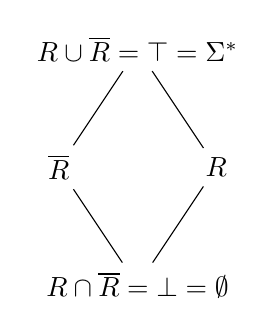
\begin{tikzpicture}
\tikzstyle{arrow} = [thick,->,>=stealth]

    \node (a) at (0,0) {$R \cup \overline{R} = \top = \Sigma^*$};
    \node (b1) at (1,-1.5) {$R$};
    \node (b2) at (-1,-1.5) {$\overline{R}$};
    \node (c) at (0,-3) {$R \cap \overline{R} = \bot = \emptyset$};
    \draw (a) to (b1);
    \draw (a) to (b2);
    \draw (b1) to (c);
    \draw (b2) to (c);
\end{tikzpicture}